% SC4013 --- Chapter 4: Broken Access Control, IDOR and Privilege Escalation (0->100)
\chapter{Broken Access Control and Privilege Escalation}\label{ch:access}
\setlength{\emergencystretch}{3em}

\begin{quote}
\emph{``Authentication is who you are; authorisation is what you may do.''} --- Most web breaches do not break the lock on the front door. They walk through an inner door that was never locked at all.
\end{quote}

\noindent\fbox{\parbox{\dimexpr\linewidth-2\fboxsep-2\fboxrule}{%
\textbf{From zero: no access-control background assumed.} We start from a hotel with key cards and master keys, then build the vocabulary of subjects, objects, permissions and policies. Every bypass---IDOR, path traversal, privilege escalation---is shown as a missing or misplaced check. Each diagram names the check that would have stopped the path.}}
\vspace{0.4em}

\section*{Learning Outcomes}
After this chapter you will be able to:
\begin{enumerate}[label=(L\arabic*)]
    \item distinguish DAC, MAC, RBAC and ABAC and choose among them;
    \item explain IDOR and demonstrate a fix with object-level authorisation;
    \item enumerate common broken-access patterns (path traversal, missing function-level checks, CORS/config);
    \item trace vertical and horizontal privilege escalation through an attack tree;
    \item enforce least privilege with deny-by-default, centralized checks and testing.
\end{enumerate}

% ============================================================
\section{Access Control in One Picture}\label{sec:models}
A \emph{subject} (user, service) requests to perform an \emph{action} (read, write, delete) on an \emph{object} (record, file, endpoint). A \emph{reference monitor} decides: allow or deny. Four classic models organise the policy:

\begin{itemize}
    \item \textbf{DAC} (Discretionary): owners set permissions (Unix \texttt{chmod}). Flexible, but permissions sprawl and leak via copy.
    \item \textbf{MAC} (Mandatory): system-wide labels decide (Bell--LaPadula). Strong, but rigid---used in military/SELinux.
    \item \textbf{RBAC} (Role-Based): users get \emph{roles} (student, instructor, admin); roles get permissions. Scales in organisations; now the dominant web model.
    \item \textbf{ABAC} (Attribute-Based): policy evaluates attributes of subject, object, action and environment (\texttt{subject.dept == object.dept AND time < 18:00}). Most expressive---used in cloud IAM and fine-grained APIs.
\end{itemize}

\begin{figure}[h]\centering
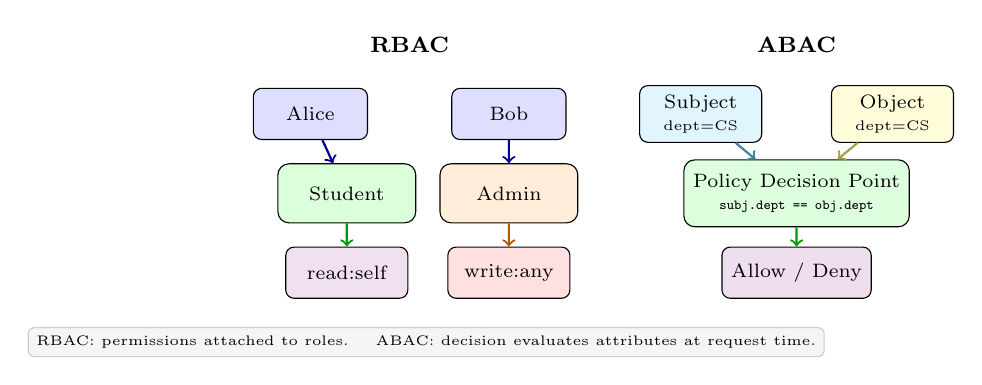
\begin{tikzpicture}[scale=0.84, every node/.style={font=\scriptsize}]
  % RBAC left
  \node[font=\footnotesize\bfseries] at (-3.2,2.9) {RBAC};
  \node[draw,fill=blue!13,rounded corners=3pt,minimum width=1.45cm,minimum height=0.65cm,align=center] (alice) at (-4.7,1.85) {Alice};
  \node[draw,fill=blue!13,rounded corners=3pt,minimum width=1.45cm,minimum height=0.65cm,align=center] (bob) at (-1.7,1.85) {Bob};
  \node[draw,fill=green!14,rounded corners=4pt,minimum width=1.75cm,minimum height=0.75cm,align=center] (roleS) at (-4.15,0.65) {Student};
  \node[draw,fill=orange!15,rounded corners=4pt,minimum width=1.75cm,minimum height=0.75cm,align=center] (roleA) at (-1.7,0.65) {Admin};
  \node[draw,fill=violet!12,rounded corners=3pt,minimum width=1.55cm,minimum height=0.65cm,align=center] (perm1) at (-4.15,-0.55) {read:self};
  \node[draw,fill=red!12,rounded corners=3pt,minimum width=1.55cm,minimum height=0.65cm,align=center] (perm2) at (-1.7,-0.55) {write:any};
  \draw[->,thick,blue!60!black] (alice) -- (roleS); \draw[->,thick,blue!60!black] (bob) -- (roleA);
  \draw[->,thick,green!60!black] (roleS) -- (perm1); \draw[->,thick,orange!70!black] (roleA) -- (perm2);
  % ABAC right
  \node[font=\footnotesize\bfseries] at (2.65,2.9) {ABAC};
  \node[draw,fill=cyan!12,rounded corners=3pt,minimum width=1.55cm,minimum height=0.65cm,align=center] (subj) at (1.2,1.85) {Subject\\ \tiny dept=CS};
  \node[draw,fill=yellow!15,rounded corners=3pt,minimum width=1.55cm,minimum height=0.65cm,align=center] (obj) at (4.1,1.85) {Object\\ \tiny dept=CS};
  \node[draw,fill=green!13,rounded corners=4pt,minimum width=2.4cm,minimum height=0.85cm,align=center] (pdp) at (2.65,0.65) {Policy Decision Point\\ \tiny \texttt{subj.dept == obj.dept}};
  \node[draw,fill=violet!13,rounded corners=3pt,minimum width=1.6cm,minimum height=0.65cm,align=center] (dec) at (2.65,-0.55) {Allow / Deny};
  \draw[->,thick,cyan!60!black] (subj) -- (pdp); \draw[->,thick,yellow!60!black] (obj) -- (pdp);
  \draw[->,thick,green!60!black] (pdp) -- (dec);
  \node[font=\tiny,fill=gray!8,draw=gray!40,rounded corners=2pt,inner sep=3pt,align=center] at (-2.95,-1.6) {RBAC: permissions attached to roles. \quad ABAC: decision evaluates attributes at request time.};
\end{tikzpicture}
\caption{RBAC versus ABAC. In RBAC the arrow from role to permission is static; in ABAC the decision point evaluates a policy over attributes of subject, object, action and environment on every request. Most real systems use RBAC for coarse roles plus ABAC rules for object-level checks.}
\label{fig:rbac-abac}
\end{figure}

All models fail the same way when the check is \emph{missing, misplaced, or uses attacker-controlled data} as the key. IDOR is the canonical example.

% ============================================================
\section{IDOR: When the Key Is in the URL}\label{sec:idor}
\emph{Insecure Direct Object Reference} means the application uses a client-supplied identifier to look up an object without verifying the caller may access that object.

\begin{lstlisting}[language=Python]
# VULNERABLE: any authenticated user can fetch any invoice by changing id
@app.route("/api/invoice/<inv_id>")
def get_invoice(inv_id):
    row = db.query("SELECT * FROM invoices WHERE id=%s", (inv_id,))
    return jsonify(row)  # no ownership check!

# FIXED: object-level authorisation -- check ownership / policy
@app.route("/api/invoice/<inv_id>")
def get_invoice_fixed(inv_id):
    row = db.query("SELECT * FROM invoices WHERE id=%s", (inv_id,))
    if row is None: abort(404)
    if row["owner_id"] != current_user.id and not current_user.is_admin:
        abort(403)  # Forbidden -- log this probe
    return jsonify(row)

# Also avoid enumerable IDs: use UUIDs or indirect reference maps
# invoice_ref = {"a7f3": 123, "b2e1": 124}  -- attacker cannot guess
\end{lstlisting}

The attack is trivial: log in as a normal user, observe \texttt{GET /api/invoice/123}, change to \texttt{124}, and read another customer's invoice. The root cause is \emph{confusing authentication with authorisation}---the endpoint checks that you are logged in, but not that you own \texttt{124}. Unenumerable IDs (UUIDs) raise the cost of guessing but do not replace the check; a single leaked URL still exposes the object.

\begin{figure}[h]\centering
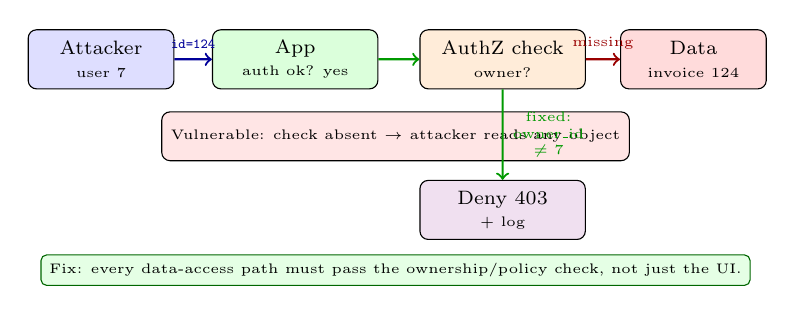
\begin{tikzpicture}[scale=0.85, every node/.style={font=\scriptsize}]
  \node[draw,fill=blue!13,rounded corners=3pt,minimum width=1.85cm,minimum height=0.75cm,align=center] (att) at (-4.5,1.6) {Attacker\\ \tiny user 7};
  \node[draw,fill=green!14,rounded corners=3pt,minimum width=2.1cm,minimum height=0.75cm,align=center] (app) at (-1.6,1.6) {App\\ \tiny auth ok? yes};
  \node[draw,fill=orange!15,rounded corners=3pt,minimum width=2.1cm,minimum height=0.75cm,align=center] (check) at (1.5,1.6) {AuthZ check\\ \tiny owner?};
  \node[draw,fill=red!14,rounded corners=3pt,minimum width=1.85cm,minimum height=0.75cm,align=center] (data) at (4.35,1.6) {Data\\ \tiny invoice 124};
  \draw[->,thick,blue!60!black] (att) -- (app) node[midway,above,font=\tiny] {\texttt{id=124}};
  \draw[->,thick,green!60!black] (app) -- (check);
  % vulnerable path
  \draw[->,thick,red!60!black] (check) -- (data) node[midway,above,font=\tiny] {missing};
  \node[draw,fill=red!10,rounded corners=3pt,minimum width=5.4cm,minimum height=0.62cm,align=center,font=\tiny] at (-0.1,0.45) {Vulnerable: check absent $\to$ attacker reads any object};
  % fixed path
  \node[draw,fill=violet!12,rounded corners=3pt,minimum width=2.1cm,minimum height=0.75cm,align=center] (deny) at (1.5,-0.65) {Deny 403\\ \tiny + log};
  \draw[->,thick,green!60!black] (check) -- (deny) node[midway,right,font=\tiny,align=center] {fixed:\\owner\_id\\$\neq$ 7};
  \node[font=\tiny,fill=green!10,draw=green!40!black,rounded corners=2pt,inner sep=3pt] at (-0.1,-1.55) {Fix: every data-access path must pass the ownership/policy check, not just the UI.};
\end{tikzpicture}
\caption{IDOR sequence: the authentication gate passes (the attacker is logged in), but the authorisation check on the \emph{object} is missing, so the request reaches data belonging to another user. The fix is a mandatory, server-side ownership check on every identifier from the client---including hidden fields, headers and batch APIs.}
\label{fig:idor-flow}
\end{figure}

{\sloppy
IDOR is not limited to numeric IDs. The same flaw appears with filenames
(\texttt{GET} \nolinkurl{/files?path=../../etc/passwd}---path traversal), API keys,
and bulk endpoints such as \texttt{POST} \nolinkurl{/api/batch} with
\texttt{\{"ids":[123,124,125]\}}. The pattern is always: client supplies a
reference, server dereferences without a policy check.\par}

% ============================================================
\section{Broken Access Control: The Wider Family}\label{sec:broken}
OWASP moved Broken Access Control to A01 in 2021 because it is both common and high-impact. Beyond IDOR:

\begin{itemize}
    \item \textbf{Missing function-level checks:} the UI hides the ``Delete user'' button, but \texttt{POST /admin/delete} is still routable and only checks ``is logged in.'' Every endpoint must enforce its policy; hiding is not enforcing.
    \item \textbf{Path traversal:} \texttt{../../../etc/passwd} escapes the intended directory when the path is concatenated. Fix: resolve, canonicalise, then verify the result is under the allowed root, or use an allow-list.
    \item \textbf{CORS and configuration:} \texttt{Access-Control-Allow-Origin: *} with \texttt{Allow-Credentials: true} lets any origin read the response; overly broad wildcard IAM policies (\texttt{s3:* on *}) turn one bug into full account compromise.
    \item \textbf{Forced browsing / method tampering:} guessing \texttt{/api/v2/admin} or switching \texttt{GET} to \texttt{PUT} bypasses a check that only covers one verb.
\end{itemize}

\begin{lstlisting}[language=Python]
# Centralised decorator: deny-by-default, one place to audit
from functools import wraps
from flask import abort, g

def require(permission):
    def deco(fn):
        @wraps(fn)
        def wrapper(*args, **kwargs):
            if not g.user or not g.user.can(permission, kwargs.get("inv_id")):
                abort(403)  # do not reveal whether object exists (403 vs 404 policy)
            return fn(*args, **kwargs)
        return wrapper
    return deco

@app.route("/api/invoice/<inv_id>", methods=["GET"])
@require("invoice:read")
def get_invoice2(inv_id):  # handler now free of scattered if-checks
    return jsonify(db.get_invoice(inv_id))
\end{lstlisting}

Centralising checks in middleware/decorators matters because scattered \texttt{if owner\_id} tests inevitably miss one path---the new mobile endpoint, the batch import, the webhook replay. Deny by default: if no rule explicitly allows, deny. Fail securely.

% ============================================================
\section{Privilege Escalation: Vertical and Horizontal}\label{sec:privesc}
\emph{Privilege escalation} is any path where an attacker gains capabilities beyond what they were granted.

\begin{figure}[h]\centering
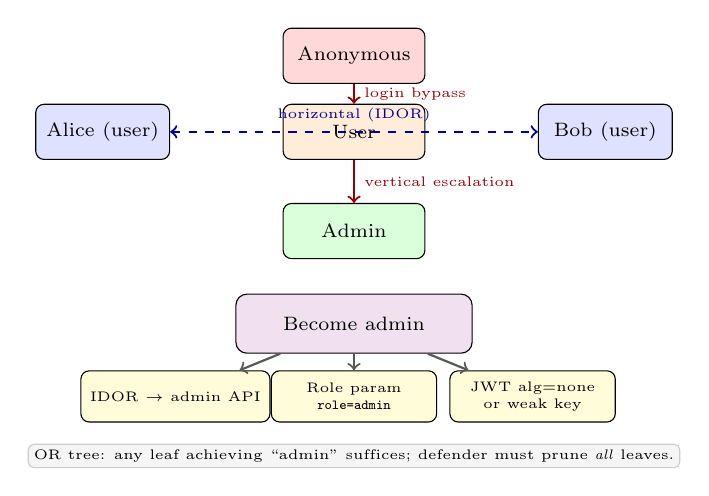
\begin{tikzpicture}[scale=0.84, every node/.style={font=\scriptsize}]
  % lattice
  \node[draw,fill=red!15,rounded corners=3pt,minimum width=1.8cm,minimum height=0.70cm,align=center] (anon) at (0,3.0) {Anonymous};
  \node[draw,fill=orange!15,rounded corners=3pt,minimum width=1.8cm,minimum height=0.70cm,align=center] (user) at (0,1.85) {User};
  \node[draw,fill=green!14,rounded corners=3pt,minimum width=1.8cm,minimum height=0.70cm,align=center] (admin) at (0,0.35) {Admin};
  \draw[->,thick,red!60!black] (anon) -- (user) node[midway,right,font=\tiny] {login bypass};
  \draw[->,thick,red!60!black] (user) -- (admin) node[midway,right,font=\tiny] {vertical escalation};
  % horizontal
  \node[draw,fill=blue!12,rounded corners=3pt,minimum width=1.7cm,minimum height=0.70cm,align=center] (uA) at (-3.8,1.85) {Alice (user)};
  \node[draw,fill=blue!12,rounded corners=3pt,minimum width=1.7cm,minimum height=0.70cm,align=center] (uB) at (3.8,1.85) {Bob (user)};
  \draw[<->,thick,blue!60!black,dashed] (uA) -- (uB) node[midway,above,font=\tiny] {horizontal (IDOR)};
  % attack tree inset
  \node[draw,fill=violet!12,rounded corners=4pt,minimum width=3.0cm,minimum height=0.75cm,align=center] (goal) at (0,-1.05) {Become admin};
  \node[draw,fill=yellow!15,rounded corners=3pt,minimum width=2.1cm,minimum height=0.65cm,align=center,font=\tiny] (a1) at (-2.7,-2.15) {IDOR $\to$ admin API};
  \node[draw,fill=yellow!15,rounded corners=3pt,minimum width=2.1cm,minimum height=0.65cm,align=center,font=\tiny] (a2) at (0,-2.15) {Role param\\ \texttt{role=admin}};
  \node[draw,fill=yellow!15,rounded corners=3pt,minimum width=2.1cm,minimum height=0.65cm,align=center,font=\tiny] (a3) at (2.7,-2.15) {JWT alg=none\\or weak key};
  \draw[->,thick,gray!70!black] (goal) -- (a1); \draw[->,thick,gray!70!black] (goal) -- (a2); \draw[->,thick,gray!70!black] (goal) -- (a3);
  \node[font=\tiny,fill=gray!8,draw=gray!40,rounded corners=2pt,inner sep=2pt,align=center] at (0,-3.05) {OR tree: any leaf achieving ``admin'' suffices; defender must prune \emph{all} leaves.};
\end{tikzpicture}
\caption{Privilege lattice and escalation tree. Horizontal movement (Alice $\leftrightarrow$ Bob) is IDOR at the same level; vertical movement (User $\to$ Admin) crosses a privilege boundary. The attack tree shows three common vertical leaves: an IDOR that reaches an admin-only object, a role parameter the server trusts, and a JWT whose signature check is bypassed. Deny-by-default and server-side role assignment prune all three.}
\label{fig:privesc}
\end{figure}

\emph{Horizontal escalation}: Alice reads Bob's data at the same privilege level (classic IDOR). \emph{Vertical escalation}: a normal user gains admin capabilities (role tampering \texttt{role=admin} in request, JWT \texttt{alg=none}, overly broad API scope, or a support endpoint that executes with service privileges). Attackers often chain: a low-severity XSS steals a session, the session reveals an IDOR, the IDOR leaks an admin token, the token yields vertical escalation.

Mitigations compose: assign roles server-side (never trust \texttt{role} from the client), validate JWT algorithm and signature with an allow-list, enforce function-level and object-level checks on every path, log every 403 (probes), and test with both positive and negative cases---``Alice must not read Bob's invoice'' is as important as ``Alice can read her own.'' Mass assignment (auto-binding) is a related trap: \texttt{user.update(request.json)} lets an attacker add \texttt{\{"is\_admin": true\}} if the framework binds all fields.

\begin{example}[Mass assignment to admin]
A profile update accepts JSON and directly maps it to the ORM: \texttt{User(**request.json).save()}. An attacker sends \texttt{\{"name":"Eve","is\_admin":true\}}. The fix is an explicit allow-list: \texttt{allowed=\{"name","email"\}; data=\{k:v for k,v in req.items() if k in allowed\}} or DTOs that expose only intended fields.
\end{example}

\begin{remark}[Least privilege end-to-end]
The application, its database role, its cloud IAM role, and its container should each have the minimum permission to function. A single IDOR then leaks one object, not the whole bucket; a single code execution runs without privilege to read secrets. Apply the same inside the app: background jobs should not run as admin, and read-only API keys should not be able to write.
\end{remark}

\begin{remark}[Auditability]
Every deny (403) should log subject, object, action and policy that denied it, with correlation IDs. During incident response those logs are the map of what the attacker probed, even when the probes failed. Without them, you cannot tell whether a missing check was exploited.
\end{remark}

% ============================================================
\section{Exercises}\label{sec:ch04-exercises}
\begin{enumerate}[label=E4.\arabic*, leftmargin=*, itemsep=0.6em]
    \item \textbf{Spot the IDOR.} Audit a tiny API (\texttt{GET /profile?id=}, \texttt{GET /orders?user=}, \texttt{POST /transfer\{to:\_, amount:\_\}}). For each endpoint list the object reference, the missing check, and a concrete curl that exploits it as user 7 reading user 8's data. Propose the fixed query + check.
    \item \textbf{Unenumerable is not auth.} A team proposes ``use UUIDs so IDs cannot be guessed'' as the sole fix for IDOR. Give a scenario where UUIDs still fail (referrer leak, log exposure, enumeration via search) and argue why an explicit ownership check is still required. When \emph{is} unenumerability a useful second layer?
    \item \textbf{Path traversal.} A file server does \texttt{open("uploads/" + filename)} where \texttt{filename} comes from the URL. Craft a payload that reads \texttt{/etc/passwd}, explain why prefixing with \texttt{"uploads/"} is insufficient, and write the canonicalise-and-verify fix in Python. How would an indirect reference map eliminate the class?
    \item \textbf{Privilege escalation tree.} Draw an attack tree for ``become admin'' on an app that (a) stores role in a JWT, (b) has \texttt{POST /api/role} hidden in the UI, and (c) serves \texttt{/admin} statically. Label each leaf with cost 1--5 and compute the cheapest path. Propose one mitigation per leaf and recompute.
    \item \textbf{Test suite design.} Design a negative-test suite for access control on an invoice resource: matrix of (anonymous, Alice, Bob, admin) $\times$ (read own, read other, delete, list all). State the expected HTTP status per cell (200/403/404) and how to avoid leaking existence via 403 vs 404. Add one test for batch \texttt{POST /invoices/export\{ids:[]\}}.
\end{enumerate}

\section*{Chapter Notes}
OWASP Top 10 A01 Broken Access Control (2021) and the OWASP Authorization Cheat Sheet are the primary references; see also OWASP Testing Guide 4.2. The RBAC model is from Ferraiolo \& Kuhn (1992); ABAC from Hu et al., NIST SP 800-162 (2014). For IDOR/path traversal labs see PortSwigger Academy (Access Control) and OWASP Juice Shop. JWT pitfalls are catalogued at \url{https://curity.io} and RFC~8725 (JWT Best Current Practices, 2020). Cloud IAM least-privilege guidance: AWS IAM Best Practices, GCP IAM Recommender, and OWASP Cloud Security.

% Additional practice: Burp Suite Intruder + Autorize extension automates IDOR discovery.
% End of Chapter 4 -- access control 200L verified
